\documentclass[a4paper]{article}

\usepackage{times}
\usepackage[T1]{fontenc}
\usepackage{a4}
\usepackage{epstopdf}
\usepackage{graphicx}
\usepackage{mathtools}
\usepackage{amssymb}  % lots of math symbols
\usepackage{hyperref}
\usepackage{color}
\usepackage{booktabs}  % nice tables

%% Unicode support
\usepackage[utf8x]{inputenc}
\usepackage{ucs}
\usepackage{autofe}

%% Code
\usepackage{minted}
\usepackage{fancyvrb}
\usepackage{inconsolata}  %% tt font
\usemintedstyle{default}

\newmint{haskell}{mathescape,fontfamily=tt}
\newmintedfile{haskell}{mathescape,fontfamily=tt}
\newminted{haskell}{gobble=8,mathescape,fontfamily=tt}

\newmint{coq}{mathescape,fontfamily=tt}
\newmintedfile{coq}{mathescape,fontfamily=tt}
\newminted{coq}{gobble=8,mathescape,fontfamily=tt}




%% Metainformation
%% PDF stuff
\usepackage{datetime}
\usepackage{ifpdf}
\ifpdf
\pdfinfo{
    /Author (Joao Paulo Pizani Flor)
    /Title (Comparing functional Embedded Domain-Specific Languages for hardware description)
    /Keywords (EDSL, HDL, Hardware Description, Functional Programming, Haskell, Coq, Lava, Coquet)
    /CreationDate (D:\pdfdate)
}
\fi

\title{Comparing functional Embedded Domain-Specific Languages for hardware description}

\date{\today}

\author
{
    João Paulo Pizani Flor \\
    Department of Information and Computing Sciences, \\
    Utrecht University - The Netherlands \\
    e-mail: j.p.pizaniflor@students.uu.nl
}



%% The document itself
\begin{document}

    \maketitle

    \section{Introduction}
    \label{sec:intro}
        Hardware design has become a very complex activity. The size of circuits has increased,
        while low-level concerns (power consumption, error correction, parallelization, layout,
        etc.) have to be incorporated earlier and earlier in the design process. This breaks
        modularity and makes it harder to validate and verify the correctness of circuits.

        In this context, researchers have been suggesting (since the 1980s) the usage of functional
        programming languages to model circuits. One particular line of research is to create
        Embedded Domain-Specific Languages for hardware description based on existing functional
        programming languages, such as Haskell.

        There are a multitude of EDSLs for hardware description, but they vary wildly
        on a number of aspects: host language, level of abstraction, capabilities of simulation,
        formal verification, synthesis (generation of netlists) and integration with other tools, to
        name a few. All this variety can make the task of choosing a hardware EDSL for the task at
        hand daunting and time-consuming.

        The main goal of this experimentation project is to establish some order in this landscape,
        and to perform a practical analysis of some popular functional hardware EDSLs. By
        reading the materials produced in this project (circuit models, test cases, generated
        netlists, report), a hardware designer wishing to use a functional hardware EDSL for his
        next design should gain some insight about the strengths and weaknesses of each language and
        have an easier time choosing one.

        As an additional result of this research, we intend to identify recent, cutting-edge
        developments in the Haskell language and its implementations from which the analyzed EDSLs
        could benefit. Also, we intend to discuss to which extent some shortcomings of the EDSLs
        could be overcome by having them hosted in a dependently-typed language.

    \section{Methodology}
    \label{sec:methods}
        In this project, we compared a number of functional hardware EDSLs that we considered
        representative (more details on the choice of EDSLs further ahead). The comparison was
        performed on a number of \emph{aspects} for each EDSL, and the analysis was done by
        considering a \emph{sample set of circuits} used as case studies.

        We tried to model all circuits in all EDSLs considered, and as similarly as possible in each
        EDSL. To avoid using any of the analyzed EDSLs as ``base'' for analysis, we provide a
        neutral, behavioural description of the circuits.

        \subsection{The languages}
        \label{subsec:languages}
            The embedded Hardware Description Languages we decided to analyze are:

            \begin{description}
                \item[Lava] The Lava\cite{lava1998} language, developed initially at Chalmers
                    University in Sweden.  Lava is deeply embedded in Haskell, and provides features
                    such as netlist generation and circuit verification using SAT-solvers. There are
                    several ``dialects'' of Lava available, and the one used for this project is
                    considered the ``canonical'' one, originally developed at Chalmers.

                \item[ForSyDe] The Haskell ForSyDe library is an EDSL based on the ``Formal System
                    Design'' approach\cite{forsyde1999}, developed at the swedish Royal Institute of
                    Technology (KTH).  It offers both shallow and deep embeddings, and provides a
                    significantly different approach to circuit modelling, using \emph{Template
                        Haskell} to allow the designer to describe combinational functions with
                    Haskell's own constructs.

                \item[Coquet] The Coquet\cite{coquet2011} EDSL differs from the other 2 mainly
                    because it's embedded in a dependently-typed programming language (the Coq theorem
                    prover). Coquet aims to allow the hardware designer to describe his circuits and
                    then \emph{interactively} prove theorems about the behaviour of whole
                    \emph{families} of circuits (using proofs by induction).
            \end{description}


        \subsection{The aspects evaluated}
        \label{subsec:aspects}
            For each of the hardware description EDSLs we experimented with, a number of
            \emph{aspects} were evaluated. The evaluated aspects do not necessarily make sense for
            \emph{all} EDSLs, therefore our presentation follows a language-centric approach, in
            which we expose the strengths and weaknesses of each EDSL concerning the applicable
            aspects.

            Without further ado, the following aspects are considered in the analysis:

            \begin{description}
                \item[Simulation]
                    The capability of simulating circuits modeled in the EDSL (and the ease with
                    which it can be performed). Simulation is understood in this context as
                    \emph{functional} simulation, i.e, obtaining the outputs calculated by the
                    circuit for certain input combinations.

                \item[Verification]
                    The capability of verifying \emph{formal properties} concerning the behaviour of
                    circuits (and the ease with which verification can be performed). The properties
                    we are interested in are those which are \emph{universally quantified} over the
                    circuit's inputs. As an example of such a property, we might have:
                    \[
                        \forall a \forall b \forall \text{\textit{sel}}
                            \left( \text{MUX}(a,b,\text{\textit{sel}}) = a \right)
                            \vee
                            \left( \text{MUX}(a,b,\text{\textit{sel}}) = b \right)
                    \]

                \item[Genericity]
                    Whether (and how well) the EDSL allows the modelling of \emph{generic} or
                    \emph{parameterized} circuits. An example of a generic circuit is a multiplexer
                    with 2 n-bit inputs and 1 n-bit output, or a multiplexer with n 1-bit inputs and
                    1 1-bit output. Besides parametrization in the \emph{size} if inputs and
                    outputs, we will also analyze whether the EDSL provides chances for
                    parametrization on other functional and/or non-functional attributes.

                \item[Depth of embedding]
                    Whether the EDSL models circuits with a \emph{shallow} embedding (using
                    predicates or functions of the host language), a \emph{deep embedding}
                    (in which circuits are members of a dedicated data type), or anything in
                    between. The depth of embedding of an EDSL might have consequences for other
                    aspects being analyzed.

                \item[Integration with other tools]
                    How well does the EDSL allow for interaction with (getting input from / generating
                    output for) other tools in the hardware design process. For example, synthesis
                    tools for FPGAs or ASICs, timing analysis tools, model checkers, etc.

                \item[Extensibility]
                    The extent to which the user can \emph{add} new interpretations, data types, and
                    combinator forms to the language. For example, the user might want to model
                    circuits that consume and produce custom datatypes, or might be interested in
                    extracting \emph{metrics} from a circuit such as power consumption, number of
                    elementary gates, etc.
            \end{description}


    \section{Modeled circuits}
    \label{sec:circuits}
        When thinking of which circuits to model using the analyzed EDSLs, some principles guided
        us. First of all, they shouldn't be too simple but also not too complex. Some very simple
        circuits (adders, counters, etc.) are very often shown as examples in the papers that define
        the EDSLs themselves, as well as in tutorials. On the other hand, we also did not want to
        model too complex circuits; that would require too much effort on the hardware design
        itself, and diverge from the focus of this project, which is to evaluate and analyze the
        EDSLs.

        Another principle that guided our choice is that the circuits should be immediately familiar
        to anyone with some minimal experience in hardware design. We avoided, therefore,
        considering application-specific circuits such as those for Digital Signal Processing (DSP),
        implementing communication protocols, etc. Having ruled out this class of circuits, we were
        left to choose from circuits that form a general-purpose computing machine, such as
        arithmetic units, memory blocks, control units and so forth.

        Finally, we wanted to choose among circuits that already had a well-defined,
        \emph{behavioural} description, to avoid using any of the analyzed EDSLs as ``basis'' of
        comparison.

        Taking these considerations into account, we chose to implement, in each of the EDSLs
        analyzed, three circuits originating from the book ``The Elements of Computing
        Systems''\cite{nand2tetris-book}. This book aims to give the reader a deep understanding of
        how computer systems work by taking a hands-on approach, in which the reader is given the
        most basic logic gates and builds, step-by-step, all the hardware and software components
        necessary to implement a complete computer system.

        From the hardware design part of the book, we took our three circuits to be modeled:

        \begin{itemize}
            \item A simple Arithmetic Logic Unit (ALU), from here onwards referred to
                as ``circuit 1''.
            \item A RAM memory block with 64 words, from here onwards referred to as ``circuit 2''.
            \item A CPU with an extremely reduced instruction set (capable of executing the
                \emph{Hack} assembly language defined in the book) from here onwards referred to as
                ``circuit 3''.
        \end{itemize}

        \subsection{Circuit 1: ALU}
        \label{subsec:circuit-alu}
            The Arithmetic Logic Unit built by us is a 2-input ALU, in which each of the inputs (as
            well as the output) is a 16-bit long word (interpreted as two's-complement signed
            integer). It is capable of computing several functions, and the choice of which
            function to compute is made by setting the ALU's 6 \emph{control bits}. To become more
            familiar with this circuit, let's first take a look at its block diagram, shown in
            figure \ref{fig:alu-block}

            \begin{figure}[h!]
                \begin{center}
                    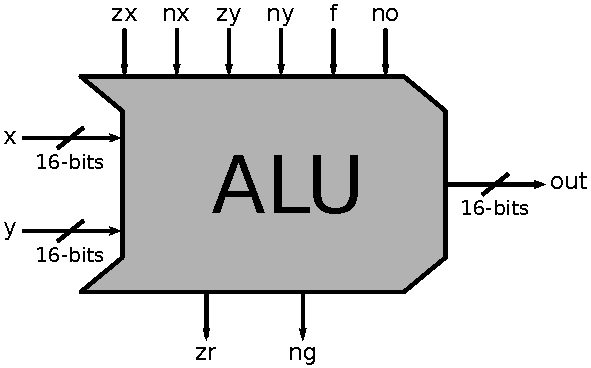
\includegraphics[width=0.55\textwidth]{imgs/alu-block.pdf}
                \end{center}
                \caption{Block diagram of circuit 1, showing its input and output ports.
                    \label{fig:alu-block}}
            \end{figure}

            Each of the 6 control bits to the ALU has, in isolation, a well-defined effect on the
            inputs or outputs to the ALU core. The bits \texttt{(zx, nx, zy, ny)} control
            ``pre-processing'' steps for the inputs \texttt{x} and \texttt{y}, with the following
            behaviour:

            \begin{description}
                \item[zx and zy] \emph{Zeroes} the x input (respectively y). The ALU core will
                    receive \texttt{0} as input.
                \item[nx and ny] Performs \emph{bitwise negation} of input x (respectively y).
            \end{description}

            Therefore, the ALU ``core'' itself (adder, and gate) has, as inputs, the results of
            performing these pre-processing steps controlled by \texttt{(zx, nx, zy, ny)}.
            Furthermore, the \emph{output} of the ALU core can also be \emph{bitwise negated} as a
            ``post-processing'' step, controlled by bit \texttt{no}.

            Finally, the control bit $f$ can be used to select which operation is to be performed by
            the ALU core: if we wish to add the two inputs, we need to set $f = 1$, and if we want
            bitwise conjunction, then we need to set $f = 0$.

            Besides the main (16-bit wide) output of the ALU, there are two other output
            \emph{flags}, that indicate predicates over the main output:

            \begin{description}
                \item[zr] Is high whenever $out = 0$.
                \item[ng] Is high whenever $out < 0$.
            \end{description}

            When the ALU is used in the context of a microprocessor these flags can be used, for
            example, to facilitate conditional jumps.

            Even though there are $2^{6} = 64$ possible combinations for the values of the control
            bits, only 18 of these combinations result in interesting functions -- that is because
            several combinations of control bits can be used to calculate the same function. We show
            these 18 functions that the ALU can calculate on table \ref{tab:alu-functions}.
            \begin{table}[h]
    \begin{center}
        \begin{tabular}{ccccccc}
            \toprule
            \textbf{zx} & \textbf{nx} & \textbf{zy} &
            \textbf{ny} & \textbf{f} & \textbf{no} & \textbf{out=}
            \tabularnewline
            \midrule

            1  &  0  &  1  &  0  &  1  &  0  &   $0$  \\

            1  &  1  &  1  &  1  &  1  &  1  &   $1$  \\

            1  &  1  &  1  &  0  &  1  &  1  &   $-1$  \\

            0  &  0  &  1  &  1  &  0  &  0  &   $x$  \\

            1  &  1  &  0  &  0  &  0  &  0  &   $y$  \\

            0  &  0  &  1  &  1  &  0  &  1  &   $\neg x$  \\

            1  &  1  &  0  &  0  &  0  &  1  &   $\neg y$  \\

            0  &  0  &  1  &  1  &  1  &  1  &   $-x$  \\

            1  &  1  &  0  &  0  &  1  &  1  &   $-y$  \\

            0  &  1  &  1  &  1  &  1  &  1  &   $x + 1$  \\

            1  &  1  &  0  &  1  &  1  &  1  &   $y + 1$  \\

            0  &  0  &  1  &  1  &  1  &  0  &   $x - 1$  \\

            1  &  1  &  0  &  0  &  1  &  0  &   $y - 1$  \\

            0  &  0  &  0  &  0  &  1  &  0  &   $x + y$  \\

            0  &  1  &  0  &  0  &  1  &  1  &   $x - y$  \\

            0  &  0  &  0  &  1  &  1  &  1  &   $y - x$  \\

            0  &  0  &  0  &  0  &  0  &  0  &   $x \wedge y$  \\

            0  &  1  &  0  &  1  &  0  &  1  &   $x \vee y$  \\

            \bottomrule
        \end{tabular}
    \end{center}
    \label{tab:alu-functions}
    \caption{Functions that the ALU can calculate, given different settings of the control bits}
\end{table}


            %% TODO: Talk about the construction of the ALU in terms of its parts.


        \subsection{Circuit 2: RAM64}
        \label{subsec:ram-circuit}
            Circuit 2 is a block of RAM with 64 lines, in which each line is a 16-bit word.
            Actually, using the term ``RAM'' to refer to this component is an abuse of terminology,
            as this circuit is nothing more than a register bank.

            All the input and output ports of the circuit are pictured in its block diagram, shown
            in figure \ref{fig:ram-block}.

            \begin{figure}[h!]
                \begin{center}
                    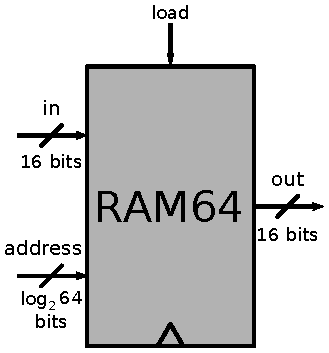
\includegraphics[width=0.5\textwidth]{imgs/ram-block.pdf}
                \end{center}
                \caption{Block diagram of circuit 2, a RAM of 64 lines
                    \label{fig:ram-block}}
            \end{figure}

            The circuit has one 16-bit output, named \texttt{out}, and three inputs (\texttt{in},
            \texttt{address} and \texttt{load}). The \texttt{in} port is 16-bit wide and holds a
            value to be written into the RAM. The \texttt{address} port has a width of $\log_{2} 64
            = 6$ bits and holds the address in which reading or writing is to be performed. Finally,
            the \texttt{load} bit controls whether the value currently at \texttt{in} should be
            written to the selected address. There is also one \emph{implicit} input for a clock
            signal in this component.  Implicit, in this case, means that the clock signal is not
            present in any of the models that we developed for this circuit, but must be present in
            any physical implementation.

            The temporal behaviour of this memory block is as follows: At any point in time, the
            output \texttt{out} holds the value stored at the memory location specified by
            \texttt{address}.  If the \texttt{load} bit is high, then the value at \texttt{in} is
            loaded into the memory word specificied by \texttt{address}. The loaded value will then
            be emitted on the output at the \textbf{next} clock cycle.

        \subsection{Circuit 3: The Hack CPU}
        \label{subsec:hack-cpu-circuit}
            Circuit 3, the largest and most complex circuit among the ones we have chosen to
            implement, is the Central Processing Unit for the \emph{Hack} computer, the machine
            described in the book ``The Elements of Computing Systems''\cite{nand2tetris-book}.

            The Hack computer is based on the \emph{Harvard architecture}, that means that it has
            different storage components and signal pathways for instructions and data. Therefore,
            the Hack CPU expects to be connected to \emph{two} memory blocks, the instruction memory
            and the data memory. Having this in mind facilitates the understanding of the CPU's
            block diagram, shown in figure \ref{fig:cpu-block}

            \begin{figure}[h!]
                \begin{center}
                    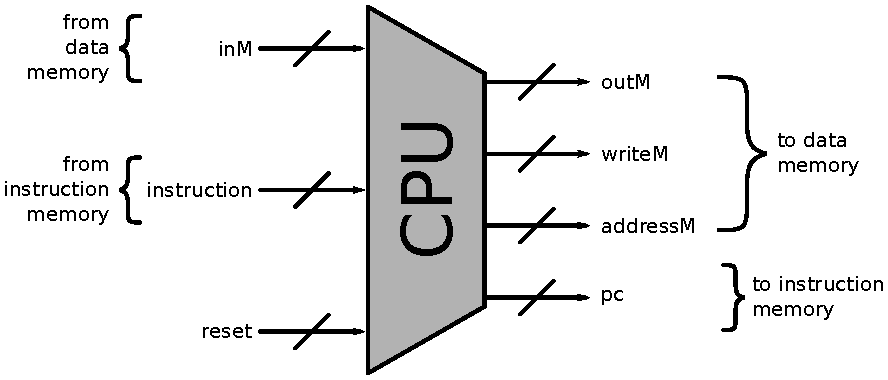
\includegraphics[width=0.9\textwidth]{imgs/cpu-block.pdf}
                \end{center}
                \caption{Block diagram of circuit 3, the Hack CPU
                    \label{fig:cpu-block}}
            \end{figure}

            The Hack architecture has an \emph{extremely} reduced instruction set, and consists in
            fact of only two instructions (each 16-bit wide): A (meaning ``address'') and
            C (meaning ''compute''). The A instruction can be used as a means to load numerical
            literals into the data memory, as well as setting a special ``cache'' register inside
            the CPU. The C instruction is the one responsible for effectively performing
            computations using the ALU, testing outputs and jumping. More details about programming
            in the Hack assembly language can be found in \cite{nand2tetris-chapter-assembly}.

            The meaning of each of the CPU's input and output ports becomes much clearer when we
            look at the context in which the CPU is inserted, namely, the memory modules to which it
            is connected. So, let's analyze the CPU's ports by taking a look at figure
            \ref{fig:cpu-memory}.

            \begin{figure}[h!]
                \begin{center}
                    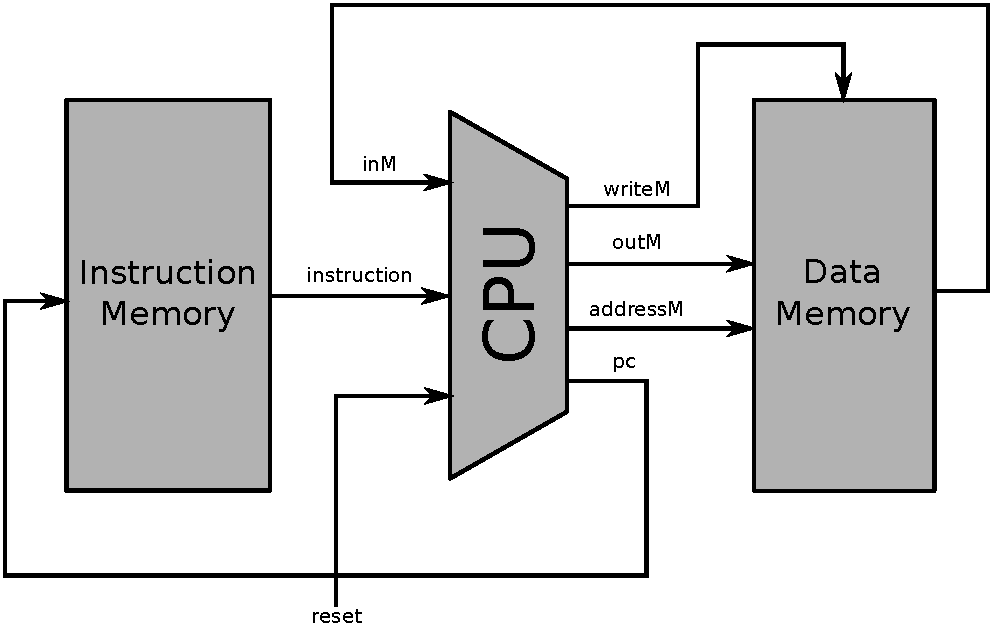
\includegraphics[width=0.9\textwidth]{imgs/cpu-memory.pdf}
                \end{center}
                \caption{The Hack CPU connected to the data and instruction memory blocks
                    \label{fig:cpu-memory}}
            \end{figure}

            Finally, the CPU is a circuit which is built mostly from the parts we already defined in
            circuits 1 and 2. We use the ALU, some registers, multiplexers, an instruction decoder
            and a counter (the \emph{program counter}). The diagram on figure \ref{fig:cpu-parts}
            shows these ``parts'' of the CPU circuit and how they are connected to each other.

            \begin{figure}[h!]
                \begin{center}
                    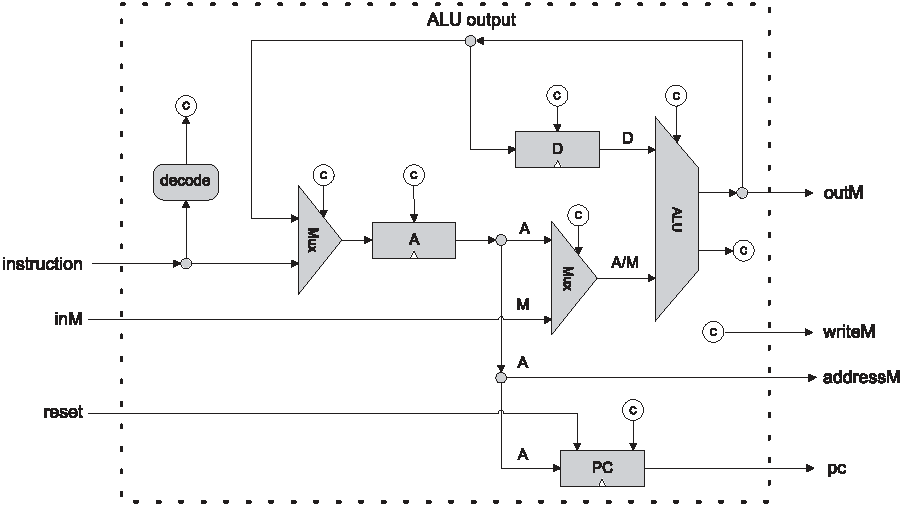
\includegraphics[width=1.0\textwidth]{imgs/cpu-parts.pdf}
                \end{center}
                \caption{Parts used in building the CPU circuit and how they are connected.
                    \label{fig:cpu-parts}}
            \end{figure}

    \section{Analysis of the EDSLs}
    \label{sec:edsls}

        \subsection{Lava}
        \label{subsec:lava}
            Lava\cite{lava1998} is an EDSL for hardware description developed originally around 1998
            at Chalmers University of Technology, in Sweden. It uses Haskell as the host language,
            and circuits described in Lava are \emph{deeply embedded}.

            The Lava EDSL has several ``dialects'', among which are Xilinx-Lava, York-Lava,
            Kansas-Lava and Chalmers-Lava. Xilinx-Lava\cite{xilinx-lava} was developed by Satnam
            Singh and puts a greater emphasis on the \emph{layout} of the described circuits,
            focusing on their implementation in Xilinx's FPGAs. York-Lava was developed as part of
            the Reduceron\cite{reduceron} project, and is a variation of Chalmers-Lava, omitting
            some features and adding some others, like a ``Prelude'' of commonly used circuits
            ((de)multiplexers, (de)coders, RAM memory blocks, etc.). Chalmers-Lava is considered the
            ``standard'' dialect, also being the one which was first developed, therefore it was
            chosen as the one to be studied in this project.

            Before diving into the inner workings of the Chalmers Lava library, we first need to
            make clear that there are two very distinct versions of this library. The original paper
            that defines the Lava language\cite{lava1998} contains the first version, while the
            current version is the one defined in a later paper\cite{observable-sharing-1999} by
            Koen Claessen and David Sands. This current version of Chalmers Lava is the one in which
            our case study is implemented.

            As already said, Lava uses a \emph{deep embedding}, and the datatype used to represent a
            circuit is \texttt{Signal}, defined in figure \ref{fig:lava-signal}. As can be noticed
            from the definition, the \emph{actual} circuit type (\texttt{S}) is ``wrapped'' around
            the \texttt{Ref} type constructor. This has to do with the approach that Lava takes to
            solving the problem of observable sharing, which is to rely on comparing
            \emph{references to object} given by the Haskell implementation, to detect cycles in
            syntax graphs representing circuits. This approach is the cause of some of Lava's
            advantages as well as disadvantages, which will be discussed further ahead.

            \begin{figure}[h!]
                \begin{center}
                    \haskellfile{code/lava-signal.hs}
                \end{center}
                \caption{Lava's \texttt{Signal} datatype, used to represent circuits.
                    \label{fig:lava-signal}}
            \end{figure}

            Having defined a circuit operating on values of a type \texttt{a} to have type
            \texttt{Signal a}, then there are several circuit combinators provided by Lava, which
            take circuits as inputs and provide circuits as outputs. For example, on figure
            \ref{fig:lava-boolean-combinators} we show some boolean circuit combinators:

            \begin{figure}[h!]
                \begin{center}
                    \haskellfile{code/lava-boolean-combinators.hs}
                \end{center}
                \caption{Some of Lava's boolean circuit combinators.
                    \label{fig:lava-boolean-combinators}}
            \end{figure}

            With Lava, one can also model circuits operating on \texttt{Int}s (and there are several
            interesting integer circuit combinators already included in the Lava library). However,
            our goal in this project was to model \emph{boolean} circuits and, besides that, integer
            circuits offer a reduced set of features.


            \subsubsection{Circuits modeled}
            \label{subsubsec:lava-circuits}
                In order to be able to describe circuit 1, the ALU (described in more detail on
                section \ref{subsec:circuit-alu}), we first needed to model the necessary
                parts. The ``core'' of the ALU is composed of a 16-bit ripple-carry adder and
                a 16-bit \texttt{AND} gate. To model the ripple-carry adder we used full adders as
                parts, which in turn used half adders. To get used to the wat in which
                circuits are described in Lava, let us first take a look at the definition of the
                hierarchy of adders in figure \ref{fig:lava-circuit1-model-adders}:

                \begin{figure}[h!]
                    \begin{center}
                        \haskellfile{code/lava-circuit1-model-adders.hs}
                    \end{center}
                    \caption{Hierarchy of adders used in circuit 1.
                        \label{fig:lava-circuit1-model-adders}}
                \end{figure}

                Based on this small model we can already make some observations concerning the
                aspects that we are analyzing. These observations are:

                \begin{itemize}
                    \item All circuits in Lava must be modeled as \emph{uncurried} functions, that
                        is, if multiple inputs are needed, they need to be packed into one tuple, the
                        same ``packing'' happens also in the case of multiple outputs.

                    \item The \emph{basic} type of input/output for all circuits modeled is
                        \texttt{Signal Bool}. This is not coincidental: Lava's VHDL generation
                        backend can only work with circuits whose input/output types are
                        \texttt{Signal Bool} or any nested combination of tuples and lists thereof.
                        This limitation makes Lava have low \textbf{extensibility}, not allowing
                        -- for example -- user-defined types.

                    \item In Lava, (families of) circuits with variable-sized inputs/outputs are
                        modeled as lists (as can be seen in the definition of
                        \texttt{rippleCarryAdder}). This approach has a good \textbf{genericity},
                        but is \textbf{not type-safe enough}. For example, we could have a circuit
                        assuming that its inputs are 32-bit wide.  There is no way to enforce, at
                        \emph{Haskell compilation time}, that inputs with correct size are
                        provided.  Possible problems could only be detected at simulation or VHDL
                        generation.
                \end{itemize}

                Now, after having defined all the necessary parts, lets take a look at the
                ALU circuit itself in figure \ref{fig:lava-circuit1-model-alu}:

                \begin{figure}[h!]
                    \begin{center}
                        \haskellfile{code/lava-circuit1-model-alu.hs}
                    \end{center}
                    \caption{Top-level model for circuit 1, the ALU.
                        \label{fig:lava-circuit1-model-alu}}
                \end{figure}

                In the definition of the ALU itself, we would like to have a user-defined datatype
                to represent the kinds of functions that can be computed by the ALU (functions
                listed on table \ref{tab:alu-functions}). However, due to the limitations of the
                VHDL backend already discussed, we have to define \texttt{ALUControlBits} as simply
                a \emph{type synonym} for a 6-tuple of bits.

                Besides modelling the three circuits in Lava, we also simulated them. The definition
                of the ALU circuit in the book "The Elements of Computing
                Systems"\cite{nand2tetris-book} has a pretty extensive truth table to test the
                circuit model, which was used to simulate the ALU. However, let's take a look at a
                simpler simulation case, that of a half-adder:
                \haskellfile{code/lava-circuit1-simulation-hadd.hs}

                Simulation of combinational circuits is performed by the Lava function
                \texttt{simulate}; it takes as arguments the circuit to simulate and an input
                combination. In the example of simulation for the \texttt{halfAdder}, we \emph{map}
                the simulation over a list of input combinations, covering all possible cases.

                The attentive reader might be asking why is this simulation not an automated test,
                i.e, why are we \textbf{not} comparing the results of the simulation with an
                \emph{expected} output sequence. This has to do with the way in which Lava handles
                the problem of observable sharing: values of type \texttt{Signal a} encapsulate
                effectively a \emph{runtime reference} to an object of type \texttt{a}. Therefore,
                even though \emph{actual} and \emph{expected} outputs might appear to be equal, they
                are considered different by Lava. Here is the offending \texttt{Eq} instance from
                the Lava library (module \texttt{Lava.Signal}):

                \begin{haskellcode}
        instance Eq (Signal a) where
            Signal (Symbol r1) == Signal (Symbol r2) = r1 == r2
                \end{haskellcode}

                With the drawback of not having \emph{automated} testing, we can say that Lava does
                provide good \textbf{simulation} capabilities, with an interface that is easy to
                understand for functional programmers.

                Now, before moving on to the next circuit
                studied, let's take a look at how Lava handles \emph{formal verification} with two
                examples: checking that a full adder is commutative and that the output of an
                incrementer circuit is always different from its input:

                \haskellfile{code/lava-circuit1-verify-fulladder.hs}

                A property over a circuit in Lava is modeled as a circuit containing \emph{one
                    boolean output}, which -- for the property to be true -- needs to be \emph{true}
                for any combination of inputs (these properties are called \emph{safety
                    properties}). Lava performs the verification by converting the circuit model to
                a CNF logical formula and executing an external SAT solver on the negation of the
                formula: the property being verified is \emph{valid} if and only if the negated
                formula is unsatisfiable. The verification for the incrementer introduces another
                detail of this kind of verification:

                \haskellfile{code/lava-circuit1-verify-incrementer.hs}

                We can see by the type of the verification function that it is a \emph{property
                    generator}, i.e, for each integer \texttt{n}, it gives a property. An
                incrementer is a circuit with generic input/output size, but the SAT-solving
                approach to verification can only prove properties for \emph{circuits of fixed
                    size}. Therefore, we can only verify a finite number of particular instances of
                the circuit.

                Moving on to circuit 2 (the RAM block), we will take a look at how Lava handles
                sequential circuits. The ``fundamental''\footnote{here, \emph{fundamental} means
                    that all sequential circuits have -- directly or indirectly -- \texttt{delay} as
                    one of its building blocks} sequential circuit in Lava is \texttt{delay}.  It
                takes two boolean signals as input and outputs a single boolean signal. Its
                semantics is that the output signal will correspond tho the input signal
                \emph{delayed} by one clock cycle, with the other parameter being the first value of
                the output.  Using this fundamental circuit, we modeled the first building block of
                our hierarchy of memory elements: a 1-bit register with input and load signals:

                \haskellfile{code/lava-circuit2-model-reg.hs}

                In this model, we use a \texttt{mux} to control whether the next state of the output
                will be simply the previous state, or the input value will be ``loaded'' into the
                register. Now, a 1-bit register can easily be ``lifted'' into a generic n-bit
                circuit:

                \haskellfile{code/lava-circuit2-model-regN.hs}

                The \texttt{regN} definition is \emph{generic}, and parameterized by the size of the
                input and output (\texttt{n}). This means that \emph{for each value of n, there is a
                    circuit \texttt{regN n}}. In Lava, however, we can only simulate and generate
                VHDL for specific instances of this family of circuits. The restriction with regards
                to VHDL generation is not a theoretical limitation, that because VHDL has good
                support for \emph{generic components}, and one could imagine Lava generating generic
                VHDL from generic circuit models. But, leaving that discussion aside, let's take a
                look at the simulation case for \texttt{regN}:

                \haskellfile{code/lava-circuit2-simulation-regN.hs}

                The \texttt{simulateSeq} function is intended for the simulation of sequential
                circuits: the list of inputs its given is the sequence of values present at the
                input ports of the circuit under test -- one element of the list for each clock
                cycle. The list of outputs given by \texttt{simulateSeq} has a similar
                interpretation.

                Having the core sequential component for our memory bank (\texttt{regN}), we modeled
                some other helper components (such as an \emph{address decoder} and a 64-to-1
                \emph{multiplexer}). With all the components at our disposal, we then modeled the
                RAM block itself:

                \haskellfile{code/lava-circuit2-model-ram64.hs}

                All the registers in the memory bank are connected to the ``global'' input word for
                the bank, but the load signal for any particular register is active \emph{iff} the
                global \texttt{load} signal is active \emph{and} (\texttt{<\&>}) that particular
                memory line is selected. Finally, to be precise, \texttt{ram64Rows} actually defines
                a family of circuits, one for each value of \texttt{n}. The one we are interested in
                is \texttt{ram64Rows 16}, for a RAM block with 64 lines, in which each line is 16
                bits wide.

                Finally, the last circuit we studied under Lava (circuit 3) is the Hack CPU
                (described in more detail on section \ref{subsec:hack-cpu-circuit}). The CPU circuit
                is mostly combinational, as it contains \emph{no form of pipelining} and
                exactly one instruction is executed per clock cycle. However, there is one
                sequential component of the CPU: the \emph{program counter}:

                \haskellfile{code/lava-circuit3-model-pc.hs}

                The program counter counts cyclically between $ 0 $ and $ 2^{n-1} $, and can have
                its value reset or set to a particular value at any moment. Having defined the
                program counter, there are still some helper parts to define before writing
                the model for the CPU itself: most importantly, we need an \emph{instruction
                    decoder}, responsible for interpreting each \texttt{Hack} instruction and
                outputting several \emph{control bits} that are used to direct the data flow inside
                the CPU during each instruction execution cycle:

                \begin{figure}[h!]
                    \begin{center}
                        \haskellfile{code/lava-circuit3-model-instruction-decoder.hs}
                    \end{center}
                    \caption{The instruction decoder of the Hack CPU.
                        \label{fig:lava-circuit3-model-decoder}}
                \end{figure}

                Here we notice again some limitations of Lava with regards to datatypes: We are
                limited to lists and tuples of \texttt{Signal Bool} (to keep the circuit
                synthesizable). Here we decided to model the \emph{Hack} instruction itself and
                the control flags as tuples, to prevent size-related runtime errors. However, using
                tuples made the model more ``cluttered'', as tuples are \emph{not} data structures
                prone to slicing and regrouping.

                Using \emph{fixed-length vectors}, perhaps based on the recent ``Type-level
                Naturals'' GHC
                \footnote{The Glorious Glasgow Haskell Compilation System:
                    \url{http://www.haskell.org/ghc}}
                extension \cite{website:ghc-typenats}
                (introduced in GHC 7.6 and being improved for GHC 7.8) would make modelling in Lava
                \emph{safer} and more comfortable.


        \subsection{ForSyDe}
        \label{subsec:forsyde}
            The Haskell ForSyDe library is an implementation of the ``Formal System Design''
            approach to hardware modelling\cite{forsyde1999}. The ForSyDe approach per se has
            several significant differences when compared to Lava, and even when the two EDSLs agree
            on \emph{what to do}, sometimes they differ on how to achieve those goals.

            To better understand what characterizes the ForSyDe methodology, we first have to
            establish some vocabulary:

            \begin{description}
                \item[System] In ForSyDe, a system or circuit is a set of processes interconnected
                    by \emph{signals}.

                \item[Signal] A signal is, intuitively, a stream of information that flows between
                    processes. It carries events of some type, and each event has an associated
                    \emph{tag}. The meaning of the tag is defined by the \emph{model of
                        computation} used.

                \item[Process] A process is nothing more than a pure function on signals. A process
                    \emph{is able} to hold internal state. But, given the same input (possibly
                    infinite) signals, it produces the same output signals.

                \item[Process constructor] Every ciruit in ForSyDe (even simplest combinational ones)
                    is built using a \emph{process constructor}. A process constructor can be seen as
                    a skeleton of behaviour, and it clearly separates computation from
                    synchronization aspects. A process constructor takes a combinational function
                    (called \emph{process function}) as parameter -- expressing the computation
                    aspect of the process, and possibly some extra values. There are combinational
                    and sequential process constructors, and some representative examples from each
                    class will be described in more detail in a specific subsection
                    (\ref{subsubsec:forsyde-synchprocs}).
            \end{description}

            \subsubsection{Models of Computation}
            \label{subsubsec:forsyde-mocs}
                The definition of signal given above is purposefully ``vague'' mainly because the
                precise definition of signals depends on the \emph{model of computation} being
                used. ForSyDe has (currently) process constructors for the following models of
                computation:

                \begin{description}
                    \item[Synchronous] All processes in this MoC have a global, implicit
                        \texttt{clock} input, and the tags in the signals are increasing natural
                        numbers. Therefore, a signal can be viewed as a \emph{stream} of values, one
                        for each clock cycle. At each clock cycle, \emph{all} processes consume
                        exactly one value from each of its inputs and produce one value at each of
                        its outputs.

                    \item[Untimed] In the untimed MoC, the processes fire individually and there is
                        no notion of global clock. A process only evaluates when its inputs have a
                        minimum number of values \emph{ready} to be read. The number of needed
                        values can vary per input, but is constant throughout execution.

                    \item[Continuous] The Continuous MoC interprets signals as continuous,
                        one-variable piecewise functions of time. It can be used to model some forms
                        of analog circuits, for example.
                \end{description}

                \label{ref:forsyde-moc-synch}
                Among all MoCs, perhaps the most ``notable'' one is the Synchronous MoC, because it
                reflects the usual interpretation of signals as wires and the vast majority of
                digital designs nowadays having a global clock. Also, all of our studied circuits
                were modelled in ForSyDe using the Synchronous MoC. Therefore, it is interesting to
                take a deeper look at it.

                First, lets take a look at the behaviour of a system which has an one integer input
                port and one integer output, and in which the value of the output is equal to the
                input plus 4. The interface and internal architecture of this system
                (\emph{addFour}) is depicted in figure \ref{fig:forsyde-addFour}.

                \begin{figure}[h!]
                    \begin{center}
                        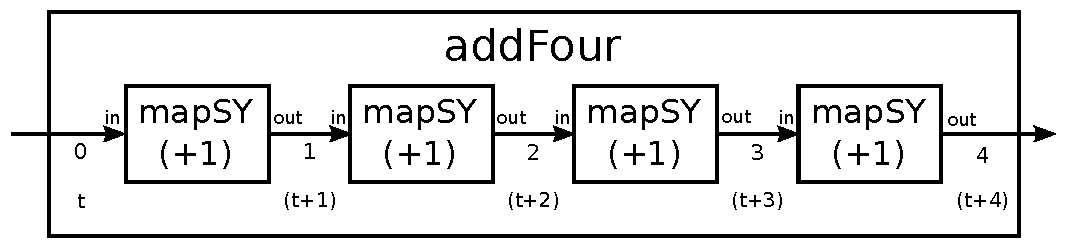
\includegraphics[width=1.0\textwidth]{imgs/forsyde-addFour.pdf}
                    \end{center}
                    \caption{The addFour circuit, example of usage of the Synchronous MoC
                        \label{fig:forsyde-addFour}}
                \end{figure}

                In this system, each of the constituent processes is built using the \texttt{mapSY}
                process constructor, a constructor of the synchronous model of computation (its name
                ends in ``SY''). It takes a combinational function (in this case ``+1'') and
                evaluates it for each event in the input signal, generating a corresponding event in
                the output signal.

                Another characteristic of ForSyDe which makes the synchronous MoC even more
                significant is that only systems that are modeled \textbf{exclusively} with process
                constructors of the synchronous model can be translated into VHDL by ForSyDe.

                ForSyDe is a \emph{deeply embedded} EDSL, but it takes a significantly different
                approach than the one taken by Lava: instead of having some set of ``atomic''
                circuits (they correspond to the constructors of the \texttt{S} type in Lava),
                ForSyDe uses Template Haskell to \emph{reify} Haskell source code into a syntax
                tree, and use this syntax tree in order to simulate and/or translate the circuit
                model into VHDL.

                On section \ref{subsec:forsyde-synchprocs} We take a closer look at synchronous
                process constructors, as well as the mechanism by which ForSyDe translates (small
                fragments of) Haskell source code into the ``building blocks'' of synchronous
                systems in VHDL.

                On section \ref{subsec:forsyde-circuits} we proceed to expose the circuits we
                modeled in ForSyDe, using the models to make a comparative analysis of ForSyDe with
                the other EDSLs.

            \subsubsection{Synchronous Process Constructors}
            \label{subsubsec:forsyde-synchprocs}
                TODO: Example of usage of \texttt{mapSY}, with a simple \texttt{ProcFun}. Mention
                that limitations to ProcFun will be discussed as the case study circuits are
                analyzed.

                In the ForSyDe Haskell package, the module \texttt{ForSyDe.Process.SynchProc}
                provides the list of process constructors that a can be used to build systems in
                ForSyDe's Synchronous Model of Computation (\ref{ref:forsyde-moc-synch}). The
                functions provided in that module can be divided in 2 big groups:

                \begin{description}
                    \item[Combinational] Combinations process constructors build processes in which
                        the value on a certain output at time $t$ depends \emph{only} on the input
                        values at time $t$. A simple example of a combinational process constructor
                        is:
                        \begin{haskellcode}
        mapSY :: (ProcType a, ProcType b) => ProcId
              -> ProcFun (a -> b) -> Signal a -> Signal b
                        \end{haskellcode}

                    \item[Sequential] On the other hand, sequential process constructors build
                        processes which can \emph{maintain state}, i.e, the value on a certain output
                        at a moment in time can depend on the value of previous inputs and outputs
                        of the circuit. A simple example of a sequential process constructor is:
                        \begin{haskellcode}
        sourceSY :: (ProcType a, ProcType b) => ProcId
                 -> ProcFun (a -> a) -> a -> Signal a
                        \end{haskellcode}

                \end{description}

                The \texttt{mapSY} constructor can be seen as the equivalent of the usual
                \texttt{map} function, but in the context of \texttt{Signal}s: For each element of
                the input signal (at each clock cycle), it applies the function to it and then
                produces as its output the result of the function application.

                Instead of being passed a ``normal'' Haskell function (with type $a → b$),
                \texttt{mapSY} is passed a \texttt{ProcFun} (Process Function). ForSyDe has
                instances of \texttt{ProcFun} which allow for it to be processed with different
                \emph{interpretations}, such as simulation, generation of VHDL or generation of
                graph diagrams. Let's take a look at how one could use the \texttt{mapSY}
                constructor to model a simple incrementer process:

                \haskellfile{code/forsyde-synchprocs-incrementer.hs}

                As already mentioned, ForSyDe makes heavy use of Template Haskell, and this example
                already clarifies how. First of all, the ``innermost'' expression
                (\verb;f x = x + 1;) is \emph{reified} by the ``\texttt{[d|}'' quasi-quoter into a
                list of declarations. This list of declarations is then transformed by
                \texttt{newProcFun} into an object of type \texttt{ExpQ} (Template Haskell's
                reified \emph{expression}). Finally, this reified expression is then
                \emph{spliced into place} and results in an object of type \texttt{ProcFun}.

                A \texttt{ProcFun} represents, intuitively, the syntax tree of the function, and
                by traversing this \texttt{ProcFun} ForSyDe can perform simulation and VHDL
                generation. There is, however, one big restriction on \texttt{ProcFun}s: As already
                seen in the type signature of \texttt{mapSY} above, the input and output types for
                the \texttt{ProcFun} have to be members of the \texttt{ProcType} class. Instances of
                \texttt{ProcType} are provided only for:

                \begin{description}
                    \item[Primitive types] \texttt{Int}, \texttt{Int8}, \texttt{Int16},
                        \texttt{Int32}, \texttt{Bool}, \texttt{ForSyDe.Bit}.
                    \item[Enumerated types] User-defined enumerations, with derived instances for
                        \texttt{Data} and \texttt{Lift}.
                    \item[Containers] Tuples and fixed-length vectors (\texttt{Data.Param.FSVec}),
                        holding a type of the above two categories and unrestrictedly nested.
                \end{description}

                For VHDL to be generated from the system definition, ForSyDe imposes a series
                of extra restrictions on the form that all \texttt{ProcFun}s can take. Upon calling
                the \texttt{writeVHDL} function, the \texttt{ProcFun} objects are traversed, and a
                \emph{runtime} error occurs if any of them does not comply with the restrictions.
                These restrictions are:

                \begin{description}
                    \item[``Point-full'' notation] Declarations with points-free notation are not
                        accepted as synthesizable
                    \item[Single-clause] To be synthesizable, a \texttt{ProcFun} cannot have
                        multiple clauses, and it cannot have \texttt{let} or \texttt{where} blocks.
                        This essentially forbids recursion inside \texttt{ProcFun}s. Pattern
                        matching is still possible by using the \texttt{case} construct.
                \end{description}

                Further details on these restrictions and how they constrain circuit design are
                shown further ahead, when analyzing the studied circuits.

                Now that the concept of a \emph{process function} is clear, let's take a look at how
                to use a sequential process constructor. In this example, we are using the
                \texttt{sourceSY} constructor to build a counter that counts in ascending order
                starting from 0:

                \begin{haskellcode}
        counter :: Signal Int16
        counter = sourceSY "counterProc" incrFunc 0
                \end{haskellcode}

                Notice that we \emph{reuse} the \texttt{incrFunc} process function, as it does
                exactly what we need. The \texttt{sourceSY} constructor takes as parameters a process
                function $f$ and an initial value $x$, and has as output signal the sequence
                $ [x, f(x), f(f(x)), f(f(f(x))), \ldots] $. This behaviour is equivalent to what the
                function \texttt{iterate} from the Haskell Prelude does.


            \subsubsection{Circuits modeled}
            \label{subsubsec:forsyde-circuits}
                Our comparative analysis of ForSyDe's strengths and weaknesses was done, as usual,
                by modelling the 3 circuits used as case-studies. ForSyDe has a peculiar ``dual''
                nature, as it supports both shallow \emph{and} deep embedded models, and models
                written with netlist generation in mind can look \emph{very} different than models
                which do not comply with the restrictions that allow synthesis.

                Because of this dual nature of ForSyDe, when modelling the case-study circuits
                we considered 2 kinds of models:

                \begin{description}
                    \item[High-level] A model that uses Haskell constructs inside the process
                        functions (\texttt{ProcFun}) as close as possible to what
                        a functional programmer would normally use. These models do not comply with
                        ForSyDe's constraints on the syntax tree of process functions for
                        synthetization, and therefore \textbf{can not be translated to VHDL}.

                    \item[Synthesizable] These models are more fine-grained, and use
                        \textbf{exclusively} constructs that allow them to be synthesized by
                        ForSyDe's VHDL backend. They ``look'' much less like functional programs and
                        more like traditional pen-and-paper diagrams of circuits.
                \end{description}

                Let's start our analysis by looking at the \emph{high-level} model for circuit 1,
                the ALU:

                \haskellfile{code/forsyde-circuit1-model-alusim.hs}

                The first thing to notice is that the system is working over \emph{16-bit integers},
                as by the definition of \texttt{WordType}. This is not exclusive of the high-level
                model, however, as ForSyDe can also produce VHDL models working with integers.

                We defined an enumeration type (\texttt{ALUOp}) that encodes possible ALU
                operations, and derived instances of the \texttt{Data} and \texttt{Lift} classes for
                it, as is required for \texttt{ALUOp} to be \texttt{ProcType}. In the body of the
                \texttt{aluFunc} process function, we perform pattern matching on the $f$ value to
                discover which operation to perform. Also, the body of \texttt{aluFunc} has a
                \texttt{where} block where all the ``parts'' that constitute the logic of the ALU
                are defined. Contrast this definition with the \emph{synthesizable} model of the
                ALU:

                \haskellfile{code/forsyde-circuit1-model-alusyn.hs}

                This model suffers from two consequences of the restrictions imposed by ForSyDe to
                enable synthesis:

                \begin{itemize}
                    \item It is too \textbf{fine grained}. As synthesizable \texttt{ProcFun}s cannot
                        have local definitions, \emph{every single} step in the datapath inside the
                        ALU has to be a process of its own.

                    \item The parallel and serial combination of processes require several steps of
                        ``zipping/unzipping'' which have nothing to do with the actual computation.
                        They only adapt the interfaces of the processes to ``fit'' together, and
                        transform between \textbf{tuples of signals and signals of tuples}. We will
                        see the same problem when handling vectors of signals.
                \end{itemize}

                An extra weakness of ForSyDe that becomes more problematic in fine-grained models is
                the need for manual \emph{name management}. Each process in ForSyDe must have a
                user-provided unique identifier: on the one hand it results in readable and modular
                VHDL netlists, but on the other hand it forces the hardware designer to work at a
                lower level than desired, making the design more error-prone.

                The issue of name management, along with the usage of fixed-length vectors, will
                become clearer as we analyze our second circuit: a RAM block of 64 lines.

                First of all, we model a n-bit register, which is not so different from the n-bit
                register we modeled in Lava:

                \haskellfile{code/forsyde-circuit2-reg.hs}

                The next needed part for the RAM is a 64-to-1 multiplexer, to choose which of the
                RAM lines to select as output, depending on the address. We modeled a whole
                hierarchy of multiplexers upto the one we needed (64-to-1): starting with a 2-to-1
                multiplexer, than building a 4-to-1 using 2-to-1 as components, 16-to-1 using 4-to-1
                and finally 64-to-1 using 16-to-1 and 4-to-1. We will only show the first two
                degress in the hierarchy:

                \haskellfile{code/forsyde-circuit2-muxes.hs}

                The hierarchy of multiplexers is a perfect example to illustrate the aforementioned
                issue of zipping/unzipping: as an input to \texttt{mux4} we get a signal of binary
                vectors (each with length 2). But we want to use \texttt{mux2} as a component,
                therefore we need to \textbf{unzip} the signal of vectors into a vector of signals,
                and then \textbf{index} the vector to get each individual signal. In the case of
                \texttt{mux16} (not shown here), this situation becomes even worse as, besides
                unzipping, we need to \textbf{re-zip} the constituent signals into ``groups'' of the
                right size to be used with the subcomponents.

                As we already mentioned, the requirement of user-given unique names for processes in
                ForSyDe results in a much more readable VHDL output for the models. Another factor
                that helps in this direction is the ForSyDe concept of \emph{component
                    instantiation}.

                When finished modelling a circuit in ForSyDe, we ``wrap it up''
                in a \emph{system definition} (a value of type \texttt{SysDef}) by calling the
                function \texttt{newSysDef}. When we call \texttt{writeVHDL} on this system
                definition, a VHDL top-level \texttt{entity} is generated. If we then want to use
                this ``finished'' model as a subcomponent in another circuit, we can use the
                \emph{instantiate} function to create a named process out of the component's
                \texttt{SysDef}. When the VHDL code for the bigger circuit is generated, the ForSyDe
                instantiation is mapped to a VHDL \texttt{component} declaration (with accompanying
                \texttt{port map} statements), which makes for pretty modular VHDL code.

                Let's now finally look at the top-level ForSyDe model for circuit 2, the RAM block:

                \haskellfile{code/forsyde-circuit2-ram.hs}

                This model is also similar to the one wrote in Lava, and that is the
                reason for why we don't have separate \emph{high-level} and \emph{synthesizable}
                models for circuit 2. The ``natural'' model, i.e, the one that came to mind
                immediately reading the description of the circuit, happens to also be
                synthesizable. In this model, we use the parts already defined before (register,
                64-to-1 multiplexer), as well as some simple gates (\texttt{and}, \texttt{or}) and
                an \emph{address decoder} (\texttt{decoder'}). We omit here the code for the address
                decoder, as it consists simply of an enumeration of all \emph{minterms} (all
                possible boolean products involving the 6 input bits and their negation).

                Lastly, let's analyze and discuss the ForSyDe model for circuit 3, the Hack CPU. We
                built the CPU using mostly already defined circuits (ALU, registers, multiplexers)
                as building blocks, which made the model also look very similar to the one written
                in Lava. This modular approach is not coincidental: in the book ``The Elements of
                Computing Systems''\cite{nand2tetris-book}, great care is taken to make each circuit
                in the hierarchy add only a small step in complexity when compared to its already
                defined subcomponents.

                In the case of the CPU, we needed to model three main additional components: a
                program counter, an instruction decoder, and a component that decides when to
                perform a jump. Let's first start by looking at the program counter:

                \haskellfile{code/forsyde-circuit3-pc.hs}

                The address type \texttt{AddrType} is defined as \texttt{Int16} because the
                specification of circuit 3 requires so. The program counter is a simple counter with
                \texttt{reset} and \texttt{set} inputs. Presenting a \texttt{high} value at the
                \texttt{reset} input will cause the program counter to output 0 at the next clock
                cycle, which will make the CPU fetch the instruction from memory address 0,
                effectively rebooting the computer. Presenting a \texttt{high} value at the
                \texttt{set} input will cause the program counter to have as its next output the
                value currently present at input \texttt{addr}. This is the way in which
                \emph{jumps} are performed in the Hack architecture.

                Having defined the model for the program counter, we proceeded to test its
                behaviour, according to the table of test cases present in chapter
                5\cite{nand2tetris-chapter-cpu} of the book defining the circuits:

                \haskellfile{code/forsyde-circuit3-pc-sim.hs}

                An important aspect of simulation with ForSyDe is that we can actually
                \emph{compare} the outputs of simulation for equality with an \emph{expected}
                sequence of inputs, which could \emph{not} be done in Lava.

                With the program counter defined and tested, we now analyze the instruction decoder:

                \haskellfile{code/forsyde-circuit3-decoder.hs}

                The job of the instruction decoder is very simple: it takes an instruction as input
                and outputs several signals to \emph{control} different parts of the CPU. It
                performs \emph{no computation} and merely \emph{rearranges} the wires. But even
                though it is such a simple circuit, the ForSyDe model is still ``ugly'' (full of
                indexing operators and tuple constructors). Because of ForSyDe's single-clause
                restriction on synthesizable \texttt{ProcFun}s, we cannot introduce a \texttt{where}
                block and give meaningful names to
                the several ``slices'' of the instruction that we are selecting.

                Now we go over the last needed subcomponent of the CPU we needed to model: a logical
                block which decides when to set the program counter and cause a jump to occur. The
                output of this circuit is connected to the \texttt{set} input of the program
                counter, as can be seen in figure \ref{fig:cpu-parts}. The code for the ForSyDe
                version of the \texttt{decideJump} block is shown below:

                \haskellfile{code/forsyde-circuit3-jump.hs}

                The decision on whether or not to perform a jump is taken based on two parameters:
                the first is a set of \texttt{jump selection bits} (named in the model as
                \texttt{JumpType}, and comes from the instruction. These bits indicate in
                \emph{which conditions} a jump is to be performed. If they are all low, then no jump
                is performed, and if they are all high, an \emph{unconditional jump} will happen.
                The second input for the \texttt{decideJump} circuit is the set of flags coming from
                the ALU. When some conditional jump is described in the \texttt{JumpType} bits, it
                will only actually happen if the correspondent ALU flags are active. The
                \texttt{decideJump} model was also tested for the input combinations described in
                the book\cite{nand2tetris-book}, but we omit the test code here for brevity.

                Having all the necessary parts we can then write the top-level model for the CPU:

                \haskellfile{code/forsyde-circuit3-cpu.hs}

                This model also looks similar to the CPU model written in Lava, but the generated
                VHDL is very different, and that is a big advantage of ForSyDe. While Lava
                \emph{flattens} all the definitions and generates \textbf{one big} VHDL entity for
                the whole model, ForSyDe is able to use the \emph{component instantiations} to
                produce a \emph{hierarchical} VHDL design, where program counter, register, ALU,
                decoder, etc., all have their \emph{own entity declarations in separate files}.

                As a closing remark on ForSyDe we can emphasize a general weakness of the library,
                which is not seen \emph{particularly} in any circuit model, but contributes to
                some of the problems discussed: ForSyDe is relatively old and not actively
                maintained. The last version available on Hackage\cite{forsyde-3.1.1-hackage} dates
                from 2010, and on the library's Hackage page there are still promises of a ``next
                version''.

                This is a problem specially because ForSyDe uses some technologies which are heavily
                dependent on GHC, and some aspects of the library could benefit from recent GHC
                developments. The \texttt{parameterized-data} package (containing the module
                \texttt{Data.Param.FSVec} of fixed-length vectors) could benefit from additions to
                the GHC type system (in particular the \texttt{TypeNats}\cite{website:ghc-typenats}
                extension) which facilitate the kind of dependent types emulated in that package.


        \subsection{Coquet}
        \label{subsec:coquet}
            The third analyzed EDSL for hardware description, Coquet\cite{coquet2011},
            is strikingly different from both others. Most of these differences can be explained in
            one way or another by its choice of host ``language'' -- Coq\footnote{``Coq'' is not
                the name of a language, but a theorem-proving system that uses different languages
                for defining terms, interactive commands, and user-defined tactics}.

            Coq is an interactive theorem prover based on \emph{intuitionistic type theory}. In the
            context of Coq, the concepts of ``term'' and ``type'' are far more intertwined than,
            say, in Haskell. Types in Coq can contain references to terms and vice-versa. A very
            typical example of these so-called \emph{dependent types} is the type(-family) of
            vectors with a certain length:

            \begin{coqcode}
        Inductive vec A : nat -> Type :=
            | nil  : vec A 0
            | cons : forall (h : A) (n : nat),  vec A n -> vec A (S n).
            \end{coqcode}

            By having the length of the vector being part of the type, we can \emph{enforce} several
            useful properties of functions operating on vectors. In fact, the type-system of Coq is
            so expressive that it can encode any proposition of \emph{intuitionistic propositional
                logic}.

            Given such expressive power, one can imagine that it might be useful to express circuits
            in Coq, and use it to prove interesting properties about these circuits. This is exactly
            the goal of Coquet. How this goal is achieved and the modelling of our studied circuits
            in Coquet is discussed in the following subsections.

            \subsubsection{Modelling circuits}
            \label{subsubsec:coquet-modelling}
                Coquet is a deep-embedded DSL, thus it represents circuits as a datatype. By using
                dependent types, a designer modelling a circuit in Coquet is able to prevent certain
                kinds of ``errors'' much earlier in the design process, because the
                \emph{well-formedness} is guaranteed by construction, i.e, every circuit built using
                the constructors provided by Coquet are well-formed by definition. Let's take a look
                at the \emph{Circuit} data type declaration:

                \begin{figure}[h!]
                    \begin{center}
                        \coqfile{code/coquet-definition-circuit.v}
                    \end{center}
                    \caption{The Circuit datatype in Coquet
                        \label{fig:coquet-circuit-type}}
                \end{figure}

                The \texttt{Circuit} type is parameterized by two types. These types are the
                \emph{input} and \emph{output} types of the circuit, respectively. They \textbf{do
                    not} represent what is ``carried'' on the wires, but the \emph{structure} of the
                circuit's input and output ports: How many of them there are, how are they grouped
                and how are they named.

                There are 2 \emph{atomic} constructors from which an element of \texttt{Circuit} can
                be built and 3 \emph{combinators}, which build a circuit based on other circuit(s).
                By observing the serial and parallel composition combinators (\texttt{Ser} and
                \texttt{Par}, respectively), we notice that the input and output types match exactly
                as expected.

                The 2 atomic constructors constrain the types \texttt{n} and \texttt{m} by requiring
                them to have instances of the ``Fin'' type class, i.e, they have to be \emph{finite}
                types (types from which a finite list of unique elements can be obtained). This
                constraint is important given the interpretation that these types (\texttt{n} and
                \texttt{m}) have: each element of \texttt{n} (respectively \texttt{m}) stands for an
                input (respectively output) ``wire'' in the circuit interface.

                The case of the ``Atom'' constructor is particularly revealing of how Coquet works:
                this constructor is parameterized by an \emph{instance} of the type class
                \texttt{Techno} for the types \texttt{n} and \texttt{m}. What this instance provides
                (in the code fragment that reads ``\texttt{techno n m}'') is the \emph{type of the
                    fundamental gate} in the technology being used. We could choose our modeled
                circuits to have, for example, NAND, NOR, or other (more exotic) gates as
                fundamental.

                As an ``usage example'' of Coquet, we show two simple circuits (\texttt{NOT} and
                \texttt{HALFADD}), along with proofs that they implement the expected functions over
                booleans. Let's start with \texttt{NOT}:

                \coqfile{code/coquet-spec-not.v}

                The input type of \texttt{NOT} is a \emph{tagged unit} with tag \texttt{x},
                similarly, the output type has tag \texttt{nx}. There is some \emph{notation}
                introduced by Coquet to make the creation of tagged units more convenient. The
                \texttt{NOT} circuit is a serial composition (denoted as \texttt{|>} of a
                \texttt{Fork2} circuit (which simply splits the input into two identical copies) and
                a \texttt{NOR} circuit, which is the underlying fundamental gate in this case.

                Below the definition of the circuit itself we state and prove the fact that our
                circuit implements the desired function (boolean negation, \texttt{negb}). More
                details on exactly what is meant by ``implements'', as well as the workings of plugs
                and tags, are exposed further ahead. Now let's take a look at a half-adder
                described in Coquet:

                \coqfile{code/coquet-spec-halfadder.v}

                First of, the sum types that are given as parameters to \texttt{Circuit} indicate
                that we have two input ports and two output ports. By using \texttt{Fork2} on a
                binary sum (\texttt{[:a] + [:b]}), we create as output a sum type in which each of
                the components is in itself a sum: that matches exactly the interface of the
                component after the \texttt{|>} operator. On the right side of the serial
                composition, we have a parallel composition of \texttt{XOR} and \texttt{AND}, giving
                two outputs: respectively the sum (\texttt{[:s]}) and carry-out (\texttt{[:c]}) 

                Together with the definition, we prove that the \texttt{HADD} circuit implements the
                boolean function we would expect, and the proof is similar to the case of
                \texttt{NOT}. It makes use of a Coquet custom tactic (\texttt{tac}), but a more
                throughout example of proof of functional correctness will be given futher ahead.
                Also, in the case of the adder used in our case study (ripple-carry adder), we prove
                that the circuit implements the \emph{actual} addition function on binary integers,
                and not some boolean equivalent.

                As a last detail on the ``user interface'' of Coquet, there is the definition of
                what exactly are the input and output types (a circuit of type \texttt{Circuit n m}
                has input type \texttt{n} and output type \texttt{m}). Usually, in the Coquet
                paper\cite{coquet2011} and in the examples provided with the library, input and
                output types are \emph{sum types} in which the terms of the sum are \emph{tagged
                    units}. Using tags serves a form of ``documentation'', giving someone reading
                the circuit model an idea of what role does each input/output port play. The
                \emph{type family} of tagged unit types is defined as follows:

                \begin{coqcode}
        Inductive tag (t : string) : Type := _tag : tag t
        Notation "[: x ]" := (tag x).
        Notation "[! x ]" := (_tag x).
        Notation "[!!]"   := (_tag _).
                \end{coqcode}

                For each string \texttt{t}, there is a type \texttt{tag t}, and this type has
                exactly one inhabitant. There are also, as part of Coquet, some definitions to make
                working with sum types less tiresome. For example, there is the function
                \texttt{sumn} which, given a type \texttt{t} and a natural \texttt{n}, returns a
                sum type with \texttt{n} elements and in which each element has type \texttt{t}.
                This might be useful if we are defining a n-bit adder:

                \begin{coqcode}
        Definition RIPPLE cin a b cout s n :
            Circuit  ([:cin] + sumn [:a] n + sumn [:b] n)  (sumn [:s] n + [:cout]) := ...
                \end{coqcode}

                While the provided examples use sums of tagged units as the input/output types, they
                can be more general: as seen in the definition of the circuit type (Fig.
                \ref{fig:coquet-circuit-type}), the only requirement is that they belong to the
                \texttt{Fin} type class, which is defined as follows:

                \begin{coqcode}
        Class Fin A := {
            eq_fin : eqT A;
            enum   : list A;
            axiom  : forall (x : A), count (equal x) enum = 1
        }.
                \end{coqcode}


            \subsubsection{Circuit semantics in Coquet}
            \label{subsubsec:coquet-semantics}
                In Coquet, the \emph{structure} and \emph{semantics} of a circuit are strictly
                separated. The structure of a circuit is modeled by a value of type
                \texttt{Circuit}, and it describes solely which are the parts that the circuit is
                make of and how they are interconnected\footnote{The \texttt{Circuit} datatype is
                    also parameterized by the type of fundamental gate used in the design.}.

                On the other hand, circuit \emph{semantics} (what operation does the circuit
                \emph{perform}) is described in Coquet by a \emph{meaning relation}. The meaning
                relation for a circuit relates its inputs to outputs, and is defined by induction on
                circuit structure.

                For a circuit type \texttt{Circuit n m} and considering \texttt{𝕋} as the type of
                what is carried in the wires, we can define the type \emph{ins} (stands for
                ``inputs'') as $n \rightarrow 𝕋$ and \emph{outs} as $m \rightarrow 𝕋$. These are
                functions that, for each input/output port, provide the a value present at that port
                -- they are in this way \emph{isomorphic} to cartesian products, and this isomorphism
                is indeed used to facilitate proofs of correctness in Coquet, as will be seen later.

                The definition of the meaning relation is as follows:

                \coqfile{code/coquet-definition-semantics.v}

                We can notice that the definition of \texttt{Semantics} has constructors that
                correspond to the constructors of \texttt{Circuit}. So, for example, given the
                semantics of two circuits \texttt{x} and \texttt{y}, we can obtain the semantics of
                their \emph{serial composition} (\texttt{Ser x y}) by using the \texttt{KSer}
                constructor. This inductive definition of semantics can also be used in proofs. If
                we need to prove a statement of the form:
                \coq;Semantics (Ser x y) ins outs;

                Then we can \texttt{apply} the \texttt{KSer} constructor to split the goal into the
                following subgoals:

                \begin{coqcode}
        Semantics x ins middles
        Semantics y middles outs
                \end{coqcode}

                While the meaning relation defines exactly the behaviour of a circuit, it is too
                low-level. We want to be able to express our \emph{specification} for circuit
                behaviour in a \emph{higher level} of abstraction -- after all, the whole point of
                proving correctness is making sure that the circuit we are modelling is
                \emph{equivalent} (in a sense) to a specification that we \emph{assume as correct}.

                Coquet offers some tools to help the user in this direction. First of all, it offers
                the designer two kinds of abstraction to facilitate writing high-level
                specifications:

                \begin{description} \item[Data abstraction] The meaning relation
                        (\texttt{Semantics}) for a circuit is a relation between two
                        \emph{functions} (\emph{ins} and \emph{outs}), which is cumbersome to reason
                        about. Therefore, Coquet allows the user to express the specification for a
                        circuit in terms of higher-level types, provided that isomorphisms between
                        these higher-level types and the function types are provided. Several
                        isomorphisms for common cases of input/output types are already provided in
                        the Coquet library, such as the isomorphism between ($ \text{sumn} \:
                        \text{\textbf{1}} \: n \rightarrow 𝔹$) and ($ 𝔹^{n} $), where \textbf{1}
                    stands for the unit type and \texttt{𝔹} for boolean).

                    \item[Behavioural abstraction] A circuit can be said to satisfy a weak
                        specification 
                        \texttt{R} if we can prove the logical entailment of \texttt{R} by the
                        meaning relation. The specification \texttt{R} already benefits from
                        \emph{data abstraction}, and ranges over the high-level types.
                \end{description}

                There are two ways to express compliance with a specification: we can say either
                that a circuit \texttt{\textbf{Realises}} a certain relation (up to isomorphisms) or
                that it \texttt{\textbf{Implements}} a certain function (up to isomorphisms). The
                difference between the \emph{relational} and the \emph{functional} models is that
                the functional model can only account for \emph{deterministic} specifications (an
                input combination maps to only one output), while with the relational model we can
                also write non-deterministic specifications. The definitions for the classes
                \texttt{Realise} and \texttt{Implement} are as follows:

                \coqfile{code/coquet-definition-realise-implement.v}

                Is we want to prove that a certain circuit \texttt{c} \emph{implements} a certain
                function \emph{f} (the high-level specification), then our goal in Coq will be:
                \coq;Implement c f; To prove this kind of statement, one can ``break down'' the
                meaning relation hypothesis, resulting in one \texttt{Semantics} hypothesis per
                circuit subcomponent.  Then the already-proven specifications of the subcomponents
                could be used to rewrite the \texttt{Semantics} hypotheses into equations. This
                makes for very modular proofs, and this will become clearer with the example proofs
                in section \ref{subsubsec:coquet-circuits}.


            \subsubsection{Circuits modeled}
            \label{subsubsec:coquet-circuits}
                TODO: Expose the studied circuits modeled in Coquet, highlighting advantages and
                disadvantages of the Coquet approach along the way.

                TODO: circuit 1 (ALU) -- Model, proof of some of its components.

                TODO: circuit 2 (RAM) -- Model.

            \subsubsection{Possible improvements and future work}
            \label{subsubsec:coquet-improv}
                The approach to circuit modelling is \emph{very} generic, and leaves room for
                extension in several aspects, even though the library is already provided with some
                reasnoable deafults.

                For example, the definition of the \emph{meaning relation} for circuits (by
                induction on circuit structure) is parameterized by the \emph{type \texttt{T} of was
                    is carried in the wires}. Even though the library already provides examples for
                booleans and streams of booleans, it could also be interesting to add cases for
                dealing with some three-valued logics, or a case for IEEE1164's std\_logic type,
                used often in VHDL.

                Another interesting point is that Coquet defines a \texttt{stream} type family, and
                then proceeds to define several interesting function over \texttt{stream}, as well
                as an instance for the meaning relation. The type family is defined as follows:

                \begin{coqcode}
        Definition stream A := nat -> A.
                \end{coqcode}

                If instead of using \texttt{nat} in the above definition, we generalized it a bit
                more (abstracting a new type parameter), we arrive at the concept of an ``event
                stream'':
                \begin{coqcode}
        Definition events tag A : tag -> A.
                \end{coqcode}
                This is exactly how ForSyDe defines its ``signals'', so we could model circuits in
                models of computation other than the synchronous model (which is the one allowed by
                the current \texttt{stream} definition).



    \section{Conclusions}
    \label{sec:conclusions}
        TODO: Reiterate the analysis of the EDSLs spread throughout the analysis of each of the
        studied circuits, but in a more summarized manner, actually \textbf{comparing} the EDSLs
        among themselves, \textbf{by aspect} (the ones we defined in section \ref{subsec:aspects}).


    \bibliographystyle{plain}
    \bibliography{references}

\end{document}
